\question 一个16端口的二层以太网交换机,冲突域和广播域的个数分别是
\par\twoch{1,1}{16,16}{1,16}{\textcolor{red}{16,1}}
\begin{solution}二层以太网交换机可以隔离冲突域,由于有16个端口,所以隔开了16个冲突域,又因为二层交换机不能隔离广播域,故只有一个广播域。
\end{solution}
\question 关于以太网交换机,下列论述中正确的是( )。 \ding{192}.交换机工作在数据链路层
\ding{193}.交换机的每个端口形成一个冲突域 \ding{194}.交换机支持多端口同时收发数据
\ding{195}.交换机是一种多端口中继器
\par\twoch{\textcolor{red}{\ding{192},\ding{193},\ding{194}}}{\ding{192},\ding{193},\ding{195}}{\ding{192},\ding{194},\ding{195}}{\ding{193},\ding{194},\ding{195}}
\begin{solution}\ding{192}:交换机是工作在数据链路层的设备,故\ding{192}正确。
\ding{193}:交换机可以隔离冲突域,但不能隔离广播域,交换机的交换结构保证了多端口同时进行数据交换,故\ding{193}正确。
\ding{194}:由\ding{193}的分析知\ding{194}正确。 \ding{195}:集线器是一种多端口的中继器,故\ding{195}错误。
\end{solution}
\question 对于使用交换机连接起来的10Mbit/s的共享式以太网,若有10个用户,则每个用户能够占有的带宽为
\par\twoch{1Mbit/s}{2Mbit/s}{\textcolor{red}{10Mbit/s}}{100Mbit/s}
\begin{solution}对于普通的10Mbit/s的共享式以太网,若有N个用户,则每个用户占有的平均带宽只有总带宽的(10Mbit/s)的N分之一。但使用以太网交换机时,虽然在每个端口到主机的带宽还是10Mbit/s,但由于一个用户在通信时是独占而不是和其他网络用户共享传输媒体的带宽,所以每个用户仍然可以得到10Mbit/s的带宽,这正是交换机的最大优点。
\end{solution}
\question 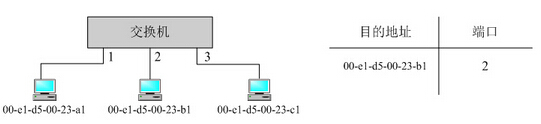
\includegraphics[width=3.33333in,height=0.76042in]{computerassets/197693a2bdb2a370018c7838bc839d05.jpeg}~

某以太网拓扑及交换机当前转发表如下图所示。主机00-e1-d5-00-23-a1向主机00-e1-d5-00-23-c1发送1个数据帧,主机00-e1-d5-00-23-c1收到该帧后,向主机00-e1-d5-00-23-a1发送1个确认帧,交换机对这两个帧的转发端口分别是(
~)
\par\fourch{{3}和{1}}{\textcolor{red}{{2,3}和{1}}}{{2,3}和{1,2}}{{1,2,3}和{1}}
\begin{solution}本题考察交换机的工作原理,开始工作时,主机a1向主机c1发送数据帧时,数据帧从1号端口发出,交换机在转发表中登记下a1的位置信息,而交换机并不知道c1连接在哪个端口下,只能向除了1号端口外的其他端口广播此数据帧,收到此数据帧的主机将数据帧中的目的地址和自己的网卡地址进行对比,如果不是发给自己的就直接丢弃,不作任何处理,而收到此数据帧的c1发现是发给自己的,此时需要向a1回复一个确认帧,注意:此时交换机是知道a1所在的端口号的,交换机在登记完c1的位置信息之后,将该确认帧直接转发到1号端口。故选项是\{2,3\}和\{1\}。
~ ~
~【总结】有些同学可能会问到:那之前题目所给的转发表信息我们不是没用到吗?既然转发表中登记了b1的位置信息,在转发a1的数据帧的时候,交换机明知道这不是给b1的分组,为何还要向他广播,这不是多此一举吗?综合前面的选择题,做到这里我们似乎能隐约看出出题人的风格了,出题人总是给我们设置一些很多具有诱惑力和迷惑性的数据,如果你对交换机的工作原理没有掌握清楚,很有可能就掉进了给你设置好的陷阱。
\end{solution}
